% HW Template for CS 6150, taken from https://www.cs.cmu.edu/~ckingsf/class/02-714/hw-template.tex
%
% You don't need to use LaTeX or this template, but you must turn your homework in as
% a typeset PDF somehow.
%
% How to use:
%    1. Update your information in section "A" below
%    2. Write your answers in section "B" below. Precede answers for all 
%       parts of a question with the command "\question{n}{desc}" where n is
%       the question number and "desc" is a short, one-line description of 
%       the problem. There is no need to restate the problem.
%    3. If a question has multiple parts, precede the answer to part x with the
%       command "\part{x}".
%    4. If a problem asks you to design an algorithm, use the commands
%       \algorithm, \correctness, \runtime to precede your discussion of the 
%       description of the algorithm, its correctness, and its running time, respectively.
%    5. You can include graphics by using the command \includegraphics{FILENAME}
%
\documentclass[11pt]{article}
\usepackage{amsmath,amssymb,amsthm}
\usepackage{graphicx}
\usepackage[margin=1in]{geometry}
\usepackage{fancyhdr}
\usepackage{algorithm}
\usepackage{algpseudocode}
\usepackage{pifont}
\setlength{\parindent}{0pt}
\setlength{\parskip}{5pt plus 1pt}
\setlength{\headheight}{13.6pt}
\newcommand\question[1]{\vspace{.25in}\hrule\textbf{#1}\vspace{.5em}\hrule\vspace{.10in}}
\renewcommand\part[1]{\vspace{.10in}\textbf{(#1)}}
\newcommand\algorith{\vspace{.10in}\textbf{Algorithm: }}
\newcommand\correctness{\vspace{.10in}\textbf{Correctness: }}
\newcommand\runtime{\vspace{.10in}\textbf{Running time: }}
\pagestyle{fancyplain}
\lhead{\textbf{\NAME\ (\UID)}}
\chead{\textbf{HW\HWNUM}}
\rhead{CS 6630, \today}
\begin{document}\raggedright
%Section A==============Change the values below to match your information==================
\newcommand\NAME{Jake Pitkin}  % your name
\newcommand\UID{u0891770}     % your utah UID
\newcommand\HWNUM{3}              % the homework number
%Section B==============Put your answers to the questions below here=======================

\question{Design One}

\textit{Overview -} My first design allows the user to visualize the political trends of a selection of states during a selected time period. The states are selected using a brush over the electoral vote chart. The time period is selected using a second brush over the year chart.

\begin{figure}[H]
  \centerline{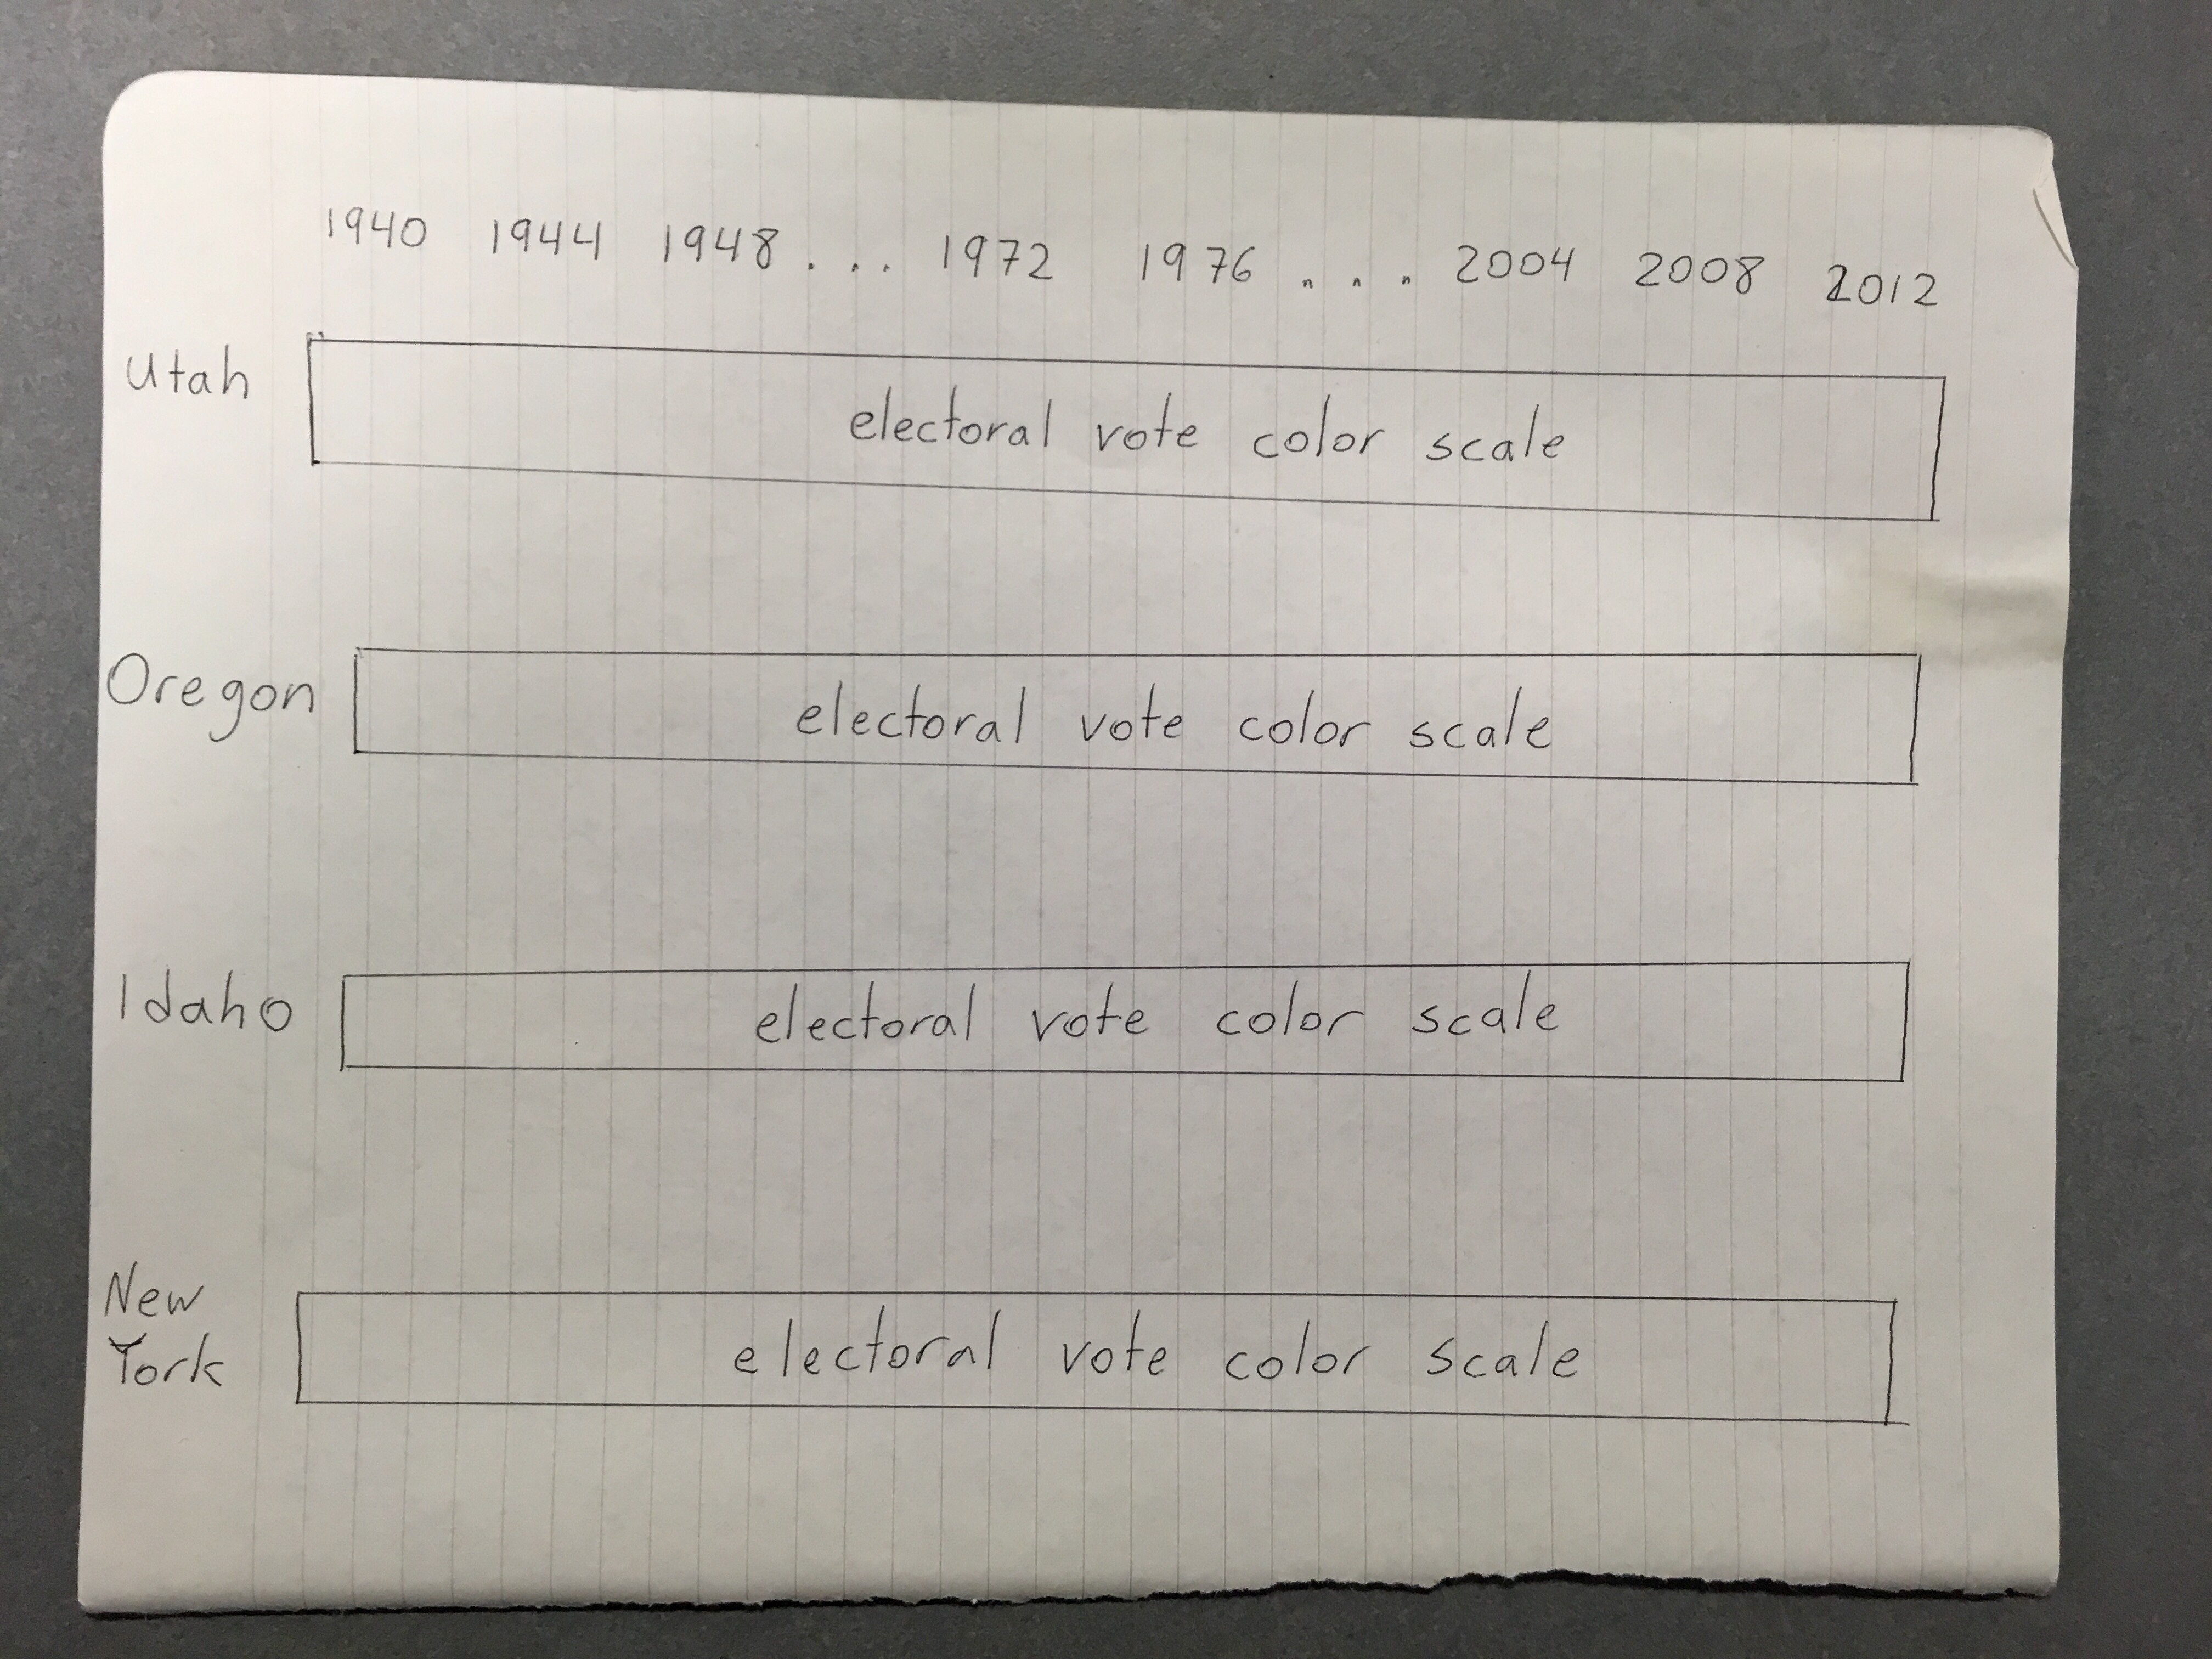
\includegraphics[width=0.5\linewidth]{design_1.jpg}}
  \caption{Stacked bar charts show political trends over time for selected states.}
\end{figure}

\textit{Marks and Channels -} Each selected state is displayed along with a stacked bar chart. The x-axis are the selected election years and each year has a fixed size rectangle in the stacked bar chart. The difference in Republican and Democratic votes is encoded using the same color scale as the electoral vote chart and the tile chart.

\textit{Pros -} Consistent with the electoral vote chart and tile chart as they both encode the same data with the same hue scale. Makes it easy to view the political shifts for an individual state. Or to compare the political trends of a small group of states. Can focus the visualization to a selected time frame.

\textit{Cons -} The current brushing method only provides the ability to compare states that are next to each other in the electoral vote chart. Additionally only consecutive election years can be selected at a given time. Not great at visualizing global trends.

\newpage

\question{Design Two}

\textit{Overview -} My second design allows the user to visualize the political trends of a selection of states during a selected time period. The states are selected using a brush over the electoral vote chart. The time period is selected using a second brush over the year chart.

\begin{figure}[H]
  \centerline{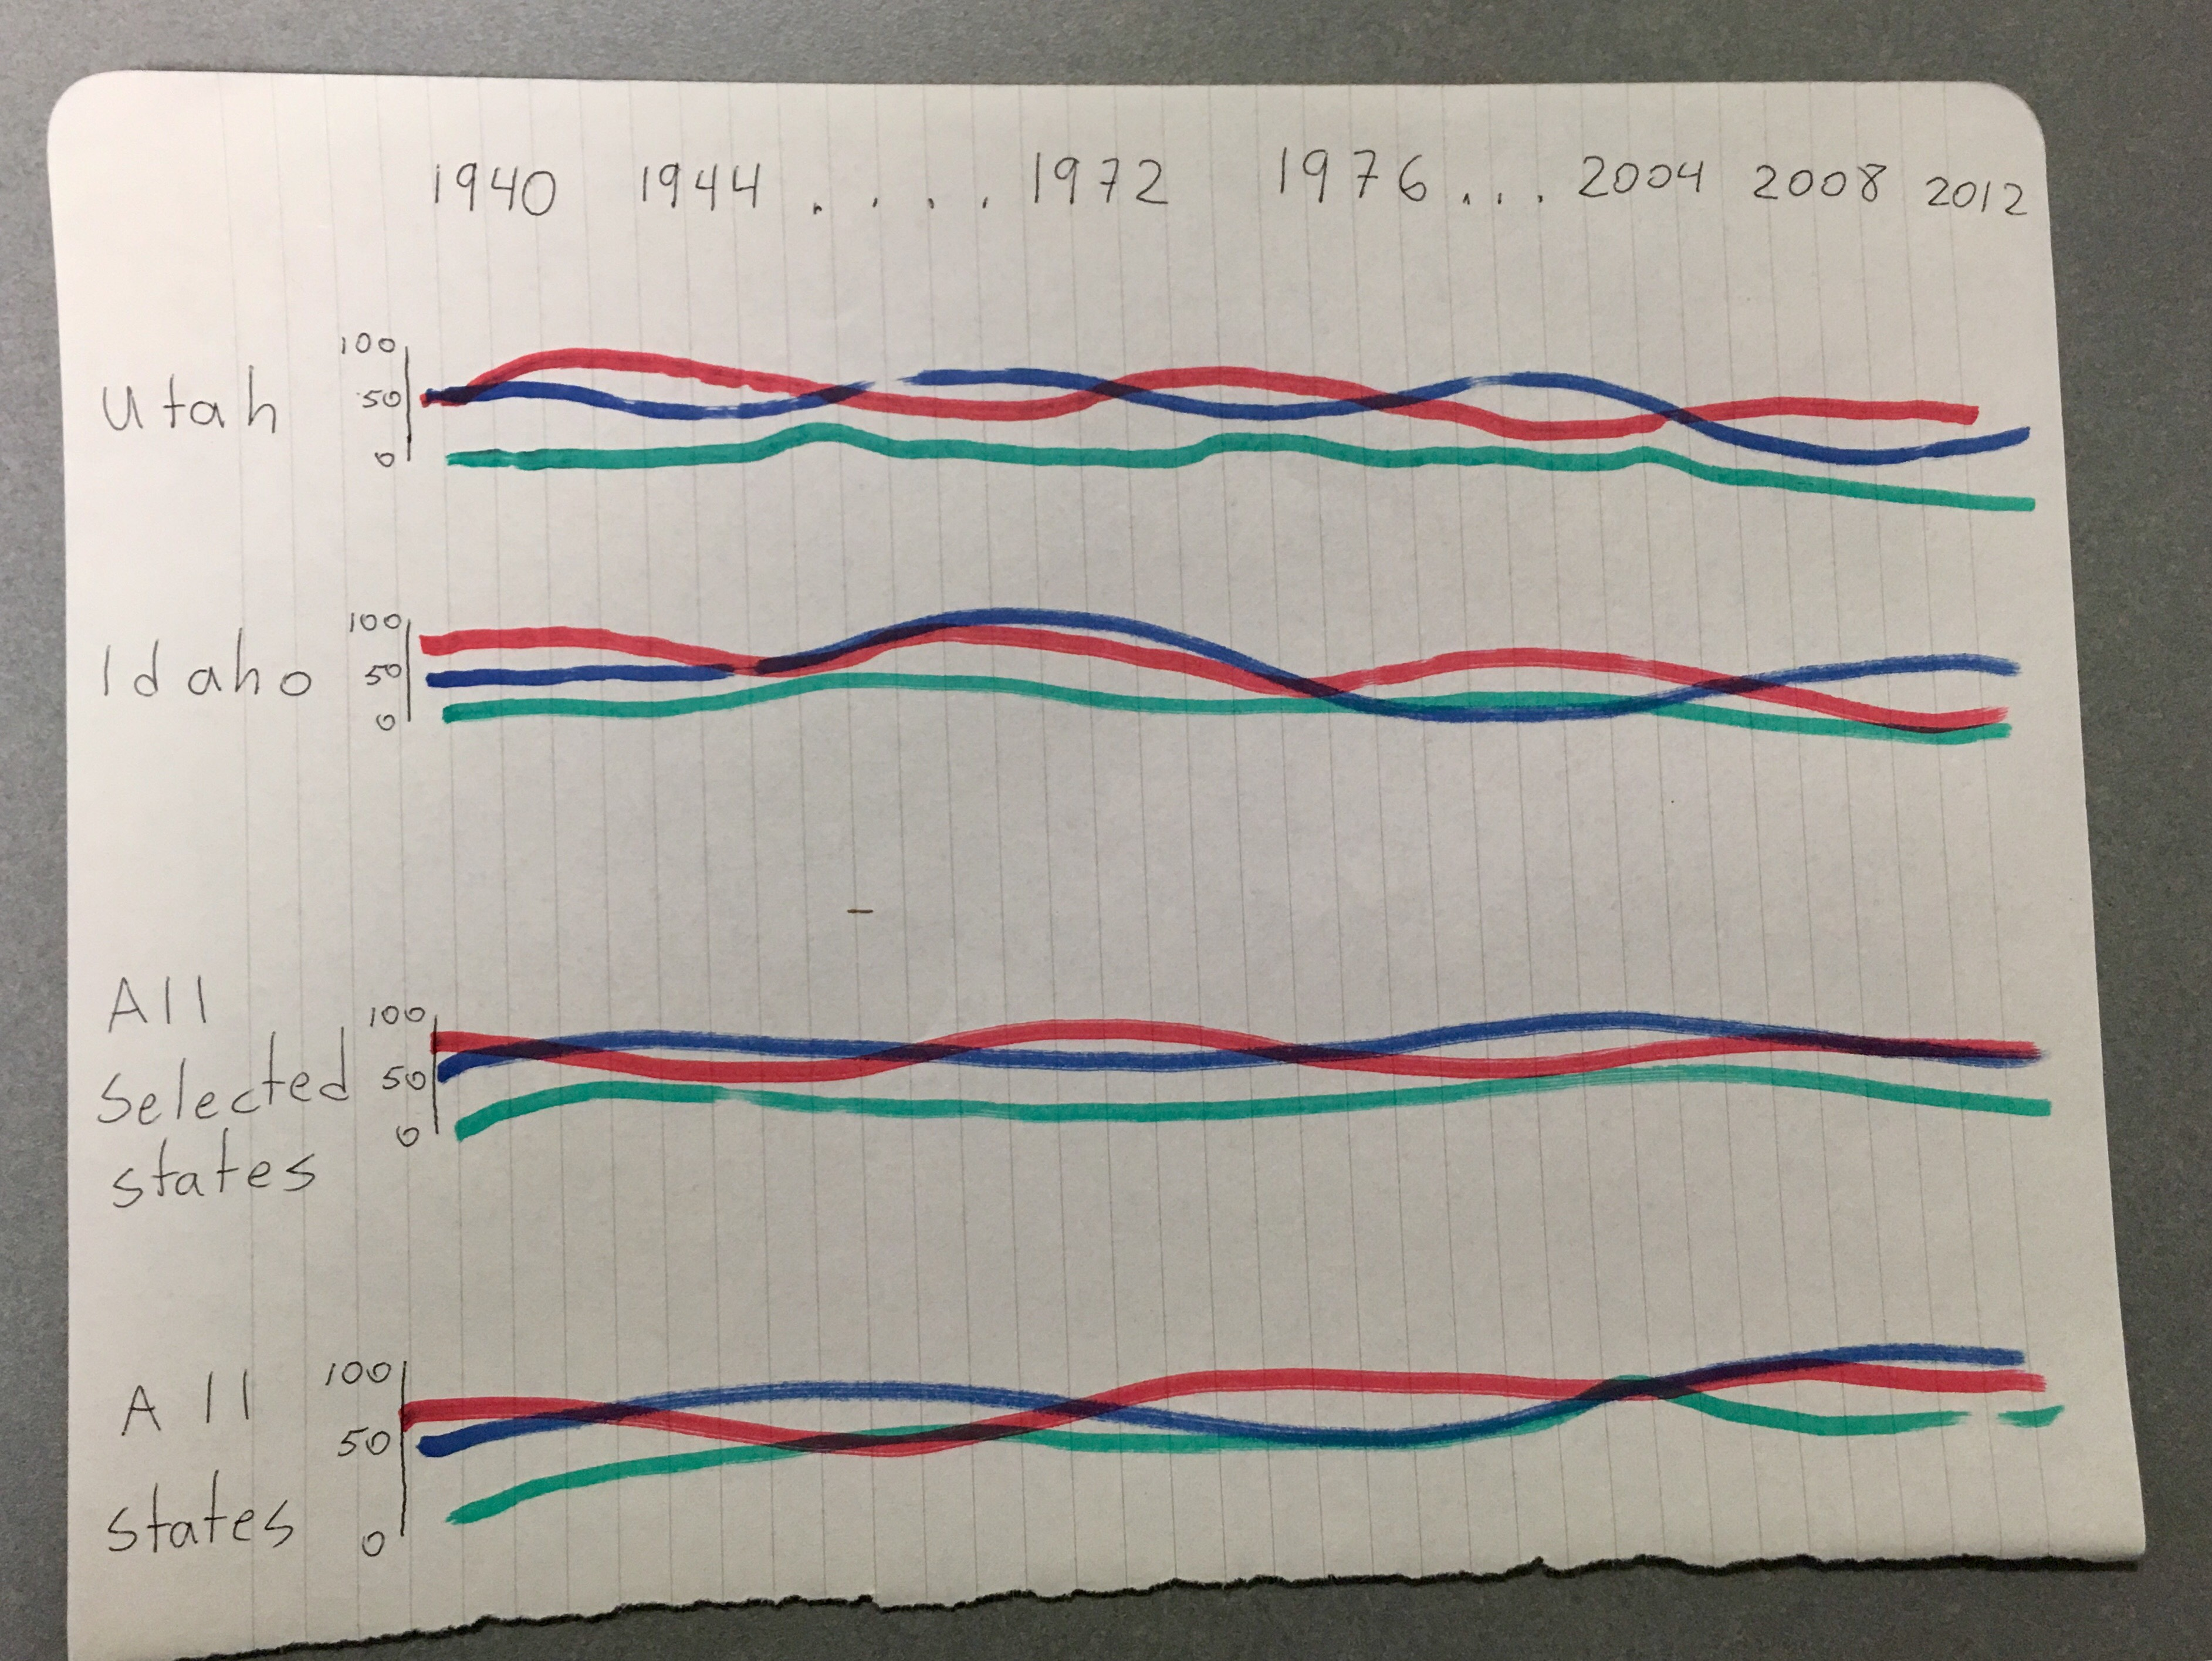
\includegraphics[width=0.5\linewidth]{design_2.jpg}}
\end{figure}

\textit{Marks and Channels -} Each selected state is displayed along with line chart consisting of three lines. Along the x-axis are the election years and along the y-axis is the percent of the electoral votes. The lines are colored to represent each of the political parties.

There are two additional line charts. One representing the aggregation of the electoral votes for all the selected states. The other the aggregation of all the states.

\textit{Pros -} Easy for a user to see a political shift between two consecutive election years for a selected state or the entire country. Can visualize what the political state was at a given time for a subset of the country.

\textit{Cons -} The current brushing method only provides the ability to compare states that are next to each other in the electoral vote chart. Additionally only consecutive election years can be selected at a given time. It's common for the Republicans and Democrats to both be close to $50\%$, which will cause a lot of overlap in the visualizations.
\end{document}